\section{Stochastic Processes}

A stochastic process is a set of random variables indexed by a parameter. If the indexing parameter is time and the random variables represent possible states then a random process describes a randomized dynamic system that reaches certain states at certain times. The formal definition of a time-indexed stochastic process is a collection $(X_t: t \in T)$ on a probability space where $t$ is the time-index and $X_t$ a random variable on the state space $S$.

A number of properties allow a more detailed classification of random processes: if the index set $T$ is countable the process is \textit{discrete} and if it is not countable the process is \textit{continuous}, if the state space $X$ is finite the process has a \textit{finite state space} and if the random variable $X_t$ represents values from a countable set the process values are \textit{discrete} and otherwise \textit{continuous}.

A common example of stochastic processes is Fractional Brownian motion as seen in Figure~\ref{fracbromotion}.

\begin{figure}
\begin{center}
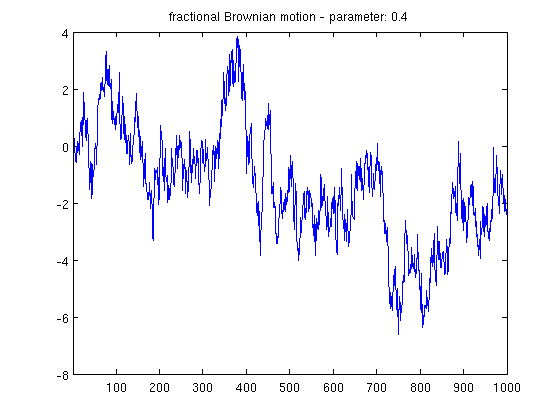
\includegraphics[height=8cm]{media/fractional_brownian_motion}\\
\end{center}
\caption{Fractional Brownian motion with Hurst parameter of $0.4$}
\label{fracbromotion}
\end{figure}

\import{src/background/stochastic_processes/}{markov_chains}
\import{src/background/stochastic_processes/}{markov_decision_processes}
\import{src/background/stochastic_processes/}{partially_observable_markov_decision_processes}